% !TEX TS-program = XeLaTeX
% !TEX spellcheck = en-US
\documentclass[aspectratio=169]{beamer}

\usetheme{example}

\title{Lecture 6:\\ Unsupervised learning}
\institute{GRA4160: Predictive modelling with machine learning}
\date{February 13th 2025}
\author{Vegard H\o ghaug Larsen}

\begin{document}

\maketitle

% Outline
\begin{frame}
\frametitle{Outline}
\begin{itemize}
    \item What is Unsupervised Learning?
    \item Dimensionality Reduction
    \item Principal Component Analysis (PCA)
    \item K-Means Clustering
    %\item Combining PCA and K-Means
    %\item Extensions and Limitations
    %\item Conclusion
\end{itemize}
\end{frame}

%--------------------------------------------------
\begin{frame}
    \frametitle{What is Unsupervised Learning?}
    \textbf{Definition:} Unsupervised Learning is a machine learning paradigm in which the model learns patterns from data that does not have labeled responses. Instead of predicting an outcome, the focus is on discovering inherent structures within the data.

    \vspace{0.5cm}
    \begin{itemize}
        \item No pre-assigned labels are needed.
        \item The goal is to uncover hidden patterns, clusters, or associations.
        \item Widely used for exploratory data analysis.
    \end{itemize}
\end{frame}
%--------------------------------------------------

%--------------------------------------------------
\begin{frame}
    \frametitle{Key Concepts in Unsupervised Learning}
    \begin{itemize}
        \item \textbf{Dimensionality Reduction:} Reducing the number of variables while preserving essential information (e.g., PCA, t-SNE).
        \item \textbf{Clustering:} Grouping data points based on similarity (e.g., K-Means, Hierarchical clustering).
        \item \textbf{Density Estimation:} Modeling the distribution of data to identify areas of high or low concentration.
        \item \textbf{Anomaly Detection:} Identifying rare items, events, or observations that raise suspicions by differing significantly from the majority.
    \end{itemize}
\end{frame}
%--------------------------------------------------

%--------------------------------------------------
\begin{frame}
    \frametitle{Comparison with Supervised Learning}
    \begin{columns}[T]
        \column{0.48\textwidth}
        \textbf{Unsupervised Learning}
        \begin{itemize}
            \item Uses unlabeled data.
            \item Focuses on pattern discovery.
            \item Commonly applied in clustering, dimensionality reduction, and anomaly detection.
        \end{itemize}

        \column{0.48\textwidth}
        \textbf{Supervised Learning}
        \begin{itemize}
            \item Uses labeled data.
            \item Focuses on prediction and classification tasks.
            \item Examples include regression, classification, and forecasting.
        \end{itemize}
    \end{columns}
\end{frame}
%--------------------------------------------------

% Introduction to Dimensionality Reduction
\begin{frame}
\frametitle{Introduction to Dimensionality Reduction}
\begin{itemize}
    \item \textbf{What?}  Reducing the number of variables/features.
    \item \textbf{Why?} The "Curse of Dimensionality" (overfitting, computation, visualization).
    \item \textbf{Benefits?} Simpler models, faster computation, visualization.
    %\item Two main approaches: Feature selection and feature extraction.
    %\item Focus: PCA (feature extraction) and K-Means (clustering).
\end{itemize}
\end{frame}

\frame{
      \frametitle{Dimensionality reduction}
      \begin{center}
            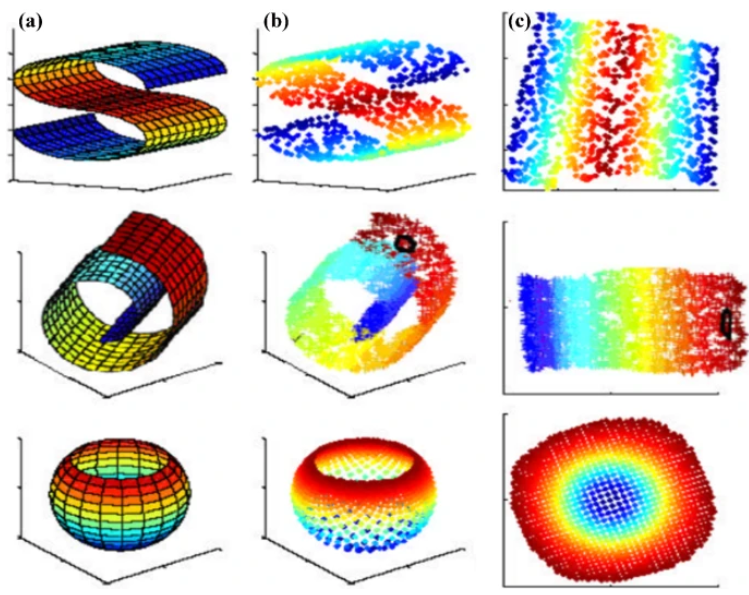
\includegraphics[width=0.5\textwidth]{figures/dim_reduction.png}\\
            \tiny{Source: \href{https://link.springer.com/article/10.1007/s40747-021-00637-x}{Link}}
      \end{center}
}

\begin{frame}\frametitle{}
    \begin{center}
        {\LARGE Principal Component Analysis (PCA)}
    \end{center}
\end{frame}

% PCA: Concept and Goal
\begin{frame}
\frametitle{Principal Component Analysis (PCA): Concept}
\begin{itemize}
    \item Linear dimensionality reduction technique.
    \item Finds new axes (principal components) that maximize variance.
    \item Can think of it as a decomposition of the data where we keep the most important information.
    \item Orthogonal components: Each captures remaining variance.
    \item Unsupervised: Ignores class labels.
    %\item Key Idea: Optimal lower-dimensional representation (maximum variance).
\end{itemize}
\end{frame}

\begin{frame}
\frametitle{PCA: Mathematical Foundation}
    \begin{itemize}
        \item \textbf{Data Preparation:} 
            \begin{itemize}
                \item Mean-centering: Subtract the mean of each feature so that the dataset is centered at the origin.
                \item Standardization: Scale features to have unit variance.
            \end{itemize}
        \item \textbf{Covariance Matrix:} 
            \[
            \Sigma = \frac{1}{n-1}X^TX
            \]
            \begin{itemize}
                \item \(X\) is the data matrix (with each row representing an observation).
                \item \(\Sigma\) captures the pairwise relationships between features.
            \end{itemize}
        \item \textbf{Eigen-decomposition:} Solve the equation:
            \[
            \Sigma \mathbf{v} = \lambda \mathbf{v}
            \]
            \begin{itemize}
                \item \(\lambda\) is an eigenvalue.
                \item \(\mathbf{v}\) is the corresponding eigenvector.
            \end{itemize}
    \end{itemize}
\end{frame}

% PCA: Mathematical Interpretation
\begin{frame}
\frametitle{PCA: Mathematical Interpretation}
    \begin{itemize}
        \item \textbf{Eigenvectors:} 
            \begin{itemize}
                \item These are special, non-zero vectors that do not change direction under the linear transformation defined by the covariance matrix \(\Sigma\).
                \item In PCA, eigenvectors indicate the directions (principal components) along which the data varies the most.
                \item They form an orthogonal basis for the feature space.
            \end{itemize}
        \item \textbf{Eigenvalues:}
            \begin{itemize}
                \item Each eigenvalue \(\lambda\) scales its corresponding eigenvector \(\mathbf{v}\).
                \item In PCA, an eigenvalue represents the variance captured along the direction of its eigenvector.
                \item A larger eigenvalue indicates a greater amount of variance along that principal component.
            \end{itemize}
    \end{itemize}
\end{frame}

\begin{frame}
    \frametitle{Eigen Decomposition: Detailed Steps}
    \begin{itemize}
        \item \textbf{Eigenvalue Equation:} $\Sigma \mathbf{v} = \lambda \mathbf{v}$
            \begin{itemize}
                \item \(\Sigma\): Covariance matrix, \(\lambda\): Eigenvalue, \(\mathbf{v}\): Eigenvector.
            \end{itemize}
        \item \textbf{Characteristic Equation:} $\det(\Sigma - \lambda I) = 0$
            \begin{itemize}
                \item This determinant yields a polynomial in \(\lambda\).
                \item The roots of this polynomial are the eigenvalues.
            \end{itemize}
        \item \textbf{Solving for Eigenvectors:}
            \begin{itemize}
                \item For each eigenvalue \(\lambda_i\), solve:
                \[
                (\Sigma - \lambda_i I)\mathbf{v}_i = \mathbf{0}
                \]
                \item This provides the corresponding eigenvector \(\mathbf{v}_i\).
            \end{itemize}
        \item \textbf{Properties:}
            \begin{itemize}
                \item Since \(\Sigma\) is symmetric, all eigenvalues are real.
                \item Eigenvectors corresponding to distinct eigenvalues are orthogonal.
            \end{itemize}
        \item \textbf{Numerical Methods:}
            \begin{itemize}
                \item For large matrices, iterative methods (e.g., QR algorithm or SVD) are used.
            \end{itemize}
    \end{itemize}
    \end{frame}
    
% PCA: Algorithm Steps
\begin{frame}
    \frametitle{PCA: Algorithm Steps}
    \begin{enumerate}
        \item \textbf{Standardize Data:} 
            \begin{itemize}
                \item \emph{Mean-center} each feature by subtracting its mean.
                \item Optionally, \emph{scale} features to have unit variance.
            \end{itemize}
        \item \textbf{Compute Covariance Matrix:}
            \[
            \Sigma = \frac{1}{n-1} X^\top X
            \]
            where \(X\) is the data matrix (each row is an observation).
        \item \textbf{Eigen-decomposition:}
            \[
            \Sigma \mathbf{v} = \lambda \mathbf{v}
            \]
            \begin{itemize}
                \item Solve for eigenvalues \(\lambda\) and eigenvectors \(\mathbf{v}\).
                \item Each eigenvector points in a direction of maximum variance.
            \end{itemize}

        \end{enumerate}
\end{frame}
    

\begin{frame}
    \frametitle{PCA: Algorithm Steps cont.}
\begin{enumerate}
\setcounter{enumi}{3}
\item \textbf{Sort Eigenpairs:}
\begin{itemize}
    \item Order the eigenpairs by descending eigenvalues.
\end{itemize}
\item \textbf{Form Projection Matrix:}
\begin{itemize}
    \item Select the top \( k \) eigenvectors.
    \item Construct the projection matrix \(\mathbf{W} \in \mathbb{R}^{d \times k}\) by using these eigenvectors as its columns.
    \item This matrix \(\mathbf{W}\) contains the \( k \) principal components.
\end{itemize}
\item \textbf{Project Data:}
\[
\mathbf{Y} = \mathbf{XW}
\]
\begin{itemize}
    \item \(\mathbf{Y}\) is the representation of the data in the reduced \( k \)-dimensional space.
\end{itemize}
\end{enumerate}
\end{frame}
    

\begin{frame}
    \frametitle{PCA: Applications and Use Cases}
    \begin{itemize}
        \item \textbf{Data Visualization (2D/3D Projections):}
            \begin{itemize}
                \item PCA reduces high-dimensional data to 2 or 3 dimensions.
                \item Facilitates the visualization of complex data structures.
                \item Helps to identify clusters, trends, and outliers visually.
            \end{itemize}
        \item \textbf{Preprocessing: Feature Reduction and Noise Filtering:}
            \begin{itemize}
                \item Reduces the number of features, making subsequent models simpler and faster.
                \item Mitigates the \emph{curse of dimensionality} by focusing on the most informative aspects of the data.
                \item Filters out noise by discarding components with low variance.
            \end{itemize}
        \item \textbf{Compression: Image Compression and Beyond:}
            \begin{itemize}
                \item \emph{Image Compression:} 
                    \begin{itemize}
                        \item In techniques like \emph{Eigenfaces}, PCA represents facial images using a reduced set of features.
                        \item Maintains essential image characteristics while significantly reducing file size.
                    \end{itemize}
                \item Useful for other data types where reducing storage and speeding up processing are crucial.
            \end{itemize}
        % \item \textbf{Applications Across Various Domains:}
        %     \begin{itemize}
        %         \item \emph{Genetics:} 
        %             \begin{itemize}
        %                 \item Analyzing genetic variations and population structure.
        %                 \item Identifying patterns in gene expression data.
        %             \end{itemize}
        %         \item \emph{Finance:} 
        %             \begin{itemize}
        %                 \item Portfolio management and risk analysis.
        %                 \item Uncovering underlying factors driving market behavior.
        %             \end{itemize}
        %         \item \emph{Computer Vision:} 
        %             \begin{itemize}
        %                 \item Enhancing facial recognition, object detection, and image segmentation.
        %             \end{itemize}
        %         \item \emph{Environmental Science:} 
        %             \begin{itemize}
        %                 \item Analyzing climate patterns and environmental datasets.
        %             \end{itemize}
        %    \end{itemize}
    \end{itemize}
    \end{frame}

    % PCA Limitations
\begin{frame}
    \frametitle{Limitations of PCA}
    \begin{itemize}
    \item \textbf{Linearity:} PCA is limited in capturing non-linear data.
    \item \textbf{Feature Scaling:} Standardization is crucial for unbiased results.
    \item \textbf{Interpretability:} Can be difficult with many features
    \item \textbf{Information Loss:} Must use explained variance to determine acceptable amount of loss.
    \item \textbf{Outliers:} Can significantly alter results.
    \end{itemize}
    \end{frame}
    

    \begin{frame}\frametitle{}
        \begin{center}
            {\LARGE K-Means Clustering}
        \end{center}
    \end{frame}

% K-Means: Concept
\begin{frame}
    \frametitle{K-Means Clustering: Concept}
    \begin{itemize}
        \item \textbf{Goal:} Partition data into \(k\) clusters such that points within each cluster are as similar as possible, while points in different clusters are as dissimilar as possible.
        \item \textbf{Centroids:} 
            \begin{itemize}
                \item Each cluster is represented by its centroid, which is the mean of the data points assigned to that cluster.
                \item The centroid is a point in the feature space that minimizes the squared distance to all points in its cluster.
            \end{itemize}
        \item \textbf{Assignment Rule:} 
            \begin{itemize}
                \item Each data point is assigned to the cluster with the nearest centroid.
                \item Distance is typically measured using the Euclidean metric.
            \end{itemize}
        \item \textbf{Hard Clustering:} 
            \begin{itemize}
                \item Each point is assigned exclusively to one cluster (no overlapping clusters or soft membership).
            \end{itemize}
    \end{itemize}
    \end{frame}
    

    \begin{frame}
        \frametitle{K-Means: Objective}
        \begin{itemize}
            \item \textbf{Objective:} Minimize the Within-Cluster Sum of Squares (WCSS)
                \begin{itemize}
                    \item Formally, the goal is to partition the data into \(k\) clusters \(\{S_1, S_2, \ldots, S_k\}\) by minimizing:
                    \[
                    \min_{S_1,\dots,S_k} \sum_{i=1}^{k} \sum_{\mathbf{x} \in S_i} \|\mathbf{x} - \mu_i\|^2,
                    \]
                    where \(\mu_i\) is the centroid (mean) of cluster \(S_i\).
                    \item This objective ensures that data points within each cluster are as close as possible to the cluster's centroid, leading to more compact and well-defined clusters.
                \end{itemize}
            \item \textbf{Centroid Definition:}
                \begin{itemize}
                    \item The centroid of a cluster \(S_i\) is computed as the mean of all data points in that cluster:
                    \[
                    \mu_i = \frac{1}{|S_i|} \sum_{\mathbf{x} \in S_i} \mathbf{x}.
                    \]
                    \item It represents the "center" of the cluster in the feature space and is used as the reference point for assigning points to clusters.
                \end{itemize}
        \end{itemize}
        \end{frame}

        \begin{frame}
            \frametitle{K-Means: Properties}
            \begin{itemize}
                \item \textbf{Convergence Properties:}
                \begin{itemize}
                    \item K-Means employs an iterative process of assigning points to the nearest centroid and then updating the centroids.
                    \item This procedure guarantees convergence to a \emph{local optimum}—the solution may depend on the initial centroid positions.
                    \item Multiple runs with different initializations (e.g., using k-means++ for better initialization) are often performed to find a more robust solution.
                \end{itemize}
            \item \textbf{Cluster Assumptions:}
                \begin{itemize}
                    \item K-Means works best when the clusters are:
                        \begin{itemize}
                            \item \textbf{Convex and roughly spherical:} The algorithm relies on Euclidean distance, which is most effective when clusters are isotropic.
                            \item \textbf{Similar in size:} Large variations in cluster size can lead to suboptimal assignments.
                        \end{itemize}
                    \item If clusters have irregular shapes or densities, alternative clustering algorithms might perform better.
                \end{itemize}
            \item \textbf{Scalability and Efficiency:}
                \begin{itemize}
                    \item K-Means is computationally efficient, making it suitable for large datasets.
                    \item However, its performance and quality of clustering can be sensitive to the number of clusters \(k\) and initial conditions.
                \end{itemize}
        \end{itemize}
\end{frame}
        

\begin{frame}
    \frametitle{K-Means: Algorithm Steps (Lloyd's Algorithm)}
    \begin{enumerate}
        \item \textbf{Initialization:}
            \begin{itemize}
                \item Choose \(k\) initial centroids.
                \item Common methods include:
                    \begin{itemize}
                        \item \emph{Random Initialization:} Select \(k\) random points from the dataset.
                        \item \emph{k-means++:} A more systematic approach that spreads out the initial centroids.
                    \end{itemize}
                \item The choice of initialization can significantly affect the final clusters.
            \end{itemize}
        \item \textbf{Assignment:}
            \begin{itemize}
                \item For each data point \(\mathbf{x}_i\), compute its distance to every centroid.
                \item Assign \(\mathbf{x}_i\) to the cluster corresponding to the nearest centroid.
                \item Typically, the Euclidean distance is used:
                \[
                \text{distance}(\mathbf{x}_i, \mu_j) = \|\mathbf{x}_i - \mu_j\|
                \]
            \end{itemize}
    \end{enumerate}
    \end{frame}
    
    \begin{frame}
        \frametitle{K-Means: Algorithm Steps (Lloyd's Algorithm) cont.}
        \begin{enumerate}
            % start counting from three
            \setcounter{enumi}{3}
            \item \textbf{Update:}
            \begin{itemize}
                \item For each cluster \(j\), recalculate the centroid \(\mu_j\) by taking the mean of all points assigned to that cluster:
                \[
                \mu_j = \frac{1}{|C_j|} \sum_{\mathbf{x}_i \in C_j} \mathbf{x}_i
                \]
                \item This step shifts the centroids to better represent the current cluster members.
            \end{itemize}
        \item \textbf{Iteration and Convergence:}
            \begin{itemize}
                \item Repeat the \emph{Assignment} and \emph{Update} steps until:
                    \begin{itemize}
                        \item The centroids do not change significantly between iterations, or
                        \item The assignments of data points to clusters stabilize, or
                        \item A maximum number of iterations is reached.
                    \end{itemize}
                \item Lloyd's algorithm is guaranteed to converge to a local optimum, though not necessarily the global optimum.
            \end{itemize}
    \end{enumerate}
    \end{frame} 

    \begin{frame}
        \frametitle{K-Means: Practical Considerations}
        \begin{itemize}
            \item \textbf{Initialization Sensitivity:}
                \begin{itemize}
                    \item The choice of initial centroids can greatly affect the convergence and final clusters.
                    \item Use \textbf{k-means++} to select well-spaced initial centroids.
                    \item Run the algorithm multiple times with different random seeds and choose the best outcome based on the objective function.
                \end{itemize}
            \item \textbf{Choosing \(k\):}
                \begin{itemize}
                    \item Use the \textbf{Elbow Method} to plot the Within-Cluster Sum of Squares (WCSS) against different values of \(k\) and identify a point of diminishing returns.
                    \item Apply \textbf{Silhouette Analysis} to assess the quality of clustering by measuring how similar an object is to its own cluster versus other clusters.
                \end{itemize}
            % \item \textbf{Feature Scaling:}
            %     \begin{itemize}
            %         \item Standardize or normalize features to ensure that each feature contributes equally.
            %         \item Prevent bias in distance calculations due to differences in feature scales.
            %     \end{itemize}
            \item \textbf{Outliers:}
                \begin{itemize}
                    \item Outliers can significantly distort centroid positions and degrade clustering quality.
                    \item Consider pre-processing steps like outlier detection or robust clustering methods.
                \end{itemize}
            %\item \textbf{Cluster Shape Assumption:}
            %    \begin{itemize}
            %        \item K-Means assumes clusters are convex and roughly spherical.
            %        \item If clusters are elongated or of irregular shape, alternative clustering methods (e.g., DBSCAN or Gaussian Mixture Models) may be more appropriate.
            %    \end{itemize}
        \end{itemize}
        \end{frame}
        

% % Choosing k
% \begin{frame}
% \frametitle{Choosing the Number of Clusters (Determining $k$)}
% \begin{itemize}
%     \item Elbow Method: Plot WCSS vs. *k*, look for "elbow".
%     \item Silhouette Analysis: Measure cluster separation.
%     \item Domain Knowledge:  Use context.
%     \item Validation:  Check for stability and meaning.
% \end{itemize}
% \end{frame}

% K-Means: Use Cases
\begin{frame}
    \frametitle{K-Means: Applications and Use Cases}
    \begin{itemize}
        \item Market segmentation.
        \item Document clustering.
        \item Image segmentation/compression.
        \item Biology and medicine.
        \item Anomaly detection (points far from centroids).
        \item General exploratory analysis.
    \end{itemize}
    \end{frame}

    % K-Means Limitations
\begin{frame}
    \frametitle{Limitations of K-Means}
    \begin{itemize}
    \item \textbf{Choosing $k$:} Requires prior knowledge of structure in the data.
    \item \textbf{Cluster shape and size:} Assumes spherical clusters of the same size.
    \item \textbf{Sensitivity to initialization:} Different starting points can lead to different results.
    \item \textbf{Outliers:} Can significantly alter cluster center points.
    \end{itemize}
    \end{frame}

% Combining PCA and K-Means
\begin{frame}
\frametitle{Combining PCA and K-Means}
\begin{itemize}
    \item PCA as preprocessing for K-Means.
    \item Benefits:
    \begin{itemize}
        \item Reduces dimensionality and noise.
        \item Speeds up K-Means.
        \item Can improve cluster quality.
        \item Facilitates visualization.
    \end{itemize}
    \item Example: Image clustering.
    \item Caution: Don't reduce dimensions \textbf{too} much.
\end{itemize}
\end{frame}

% % Extensions and Variants
% \begin{frame}
% \frametitle{Extensions and Variants of PCA and K-Means}
% \begin{itemize}
%     \item PCA: Kernel PCA, Sparse PCA, Incremental PCA.
%     \item K-Means: K-Means++, K-Medoids, Fuzzy C-Means, Hierarchical Clustering, Gaussian Mixture Models, DBSCAN.
% \end{itemize}
% \end{frame}


% Conclusion
\begin{frame}
\frametitle{Conclusion}
\begin{itemize}
    \item \textbf{PCA:} Dimensionality reduction, maximizes variance.
    \item \textbf{K-Means:} Clustering, minimizes within-cluster variance.
    \item \textbf{Use PCA for:} High-dimensional data, visualization, noise reduction.
    \item \textbf{Use K-Means for:}  Finding groups, exploratory analysis.
    \item \textbf{Powerful combination:} PCA + K-Means.
    %\item Be aware of limitations and consider extensions.
\end{itemize}
\end{frame}

% \begin{frame}
% \frametitle{References}
% \footnotesize
% \begin{itemize}
%     \item Wikipedia: Principal Component Analysis, K-means Clustering
%     \item Sebastian Raschka (2015): PCA in 3 Steps
%     \item IBM Cloud Learn Hub: What is K-Means Clustering?
%     \item DataCamp Blog (2023): The Curse of Dimensionality in Machine Learning
%     \item Stack Exchange (Cross Validated)
%     \item Brunton et al. (2015): Eigenfaces example

% \end{itemize}

% \end{frame}

\end{document}